
\documentclass{sig-alternate}
\usepackage{mdwlist}
\usepackage{url}
\usepackage{graphicx}

\begin{document} 

\title{Automatic Harmonization}
\subtitle{Viewed as a Machine Translation Problem}
\numberofauthors{2}
\author{
\alignauthor Nicole Limtiaco \\ \email{limni@seas.upenn.edu} \\ Univ. of Pennsylvania \\ Philadelphia, PA
\alignauthor Rigel Swavely \\ \email{rigel@seas.upenn.edu} \\ Univ. of Pennsylvania \\ Philadelphia, PA}
\date{}
\maketitle

\begin{abstract}
  \textit{In the past, approaches to automatic harmonization of a melody
  have taken two forms: using rules provided by music theory or by predicting
  the chord under the melody. This attempt approaches the problem from a machine translation perspective, 
  modeling the melody of a song as the source language and each harmony as a target language.
  By generating the harmony lines explicitly rather that generating them as a
  consequence of the chord on each beat, we hope that the algorithm will be able to create
  more cohesive, creative works.}

  \textit{In order to accomplish this, we will create a translation model to represent the probability
  of one note harmonizing with another note. Additionally, we will create a language model to represent
  a note following a phrase of notes in the same line of music. A perplexity metric will be used to 
  evaluate the performance of our algorithm. If there is time, we hope to incorporate human evaluation
  and data driven rhythmic variation.}
\end{abstract}

\section{Introduction}
\label{sec:intro}
Many would consider music composition to be an art form that is accomplished
primarily through human creativity. Writing music is a process that seems to require
complex thought which fundamentally cannot be boiled down to a list of straightforward
processes. Our project aims to answer the question, ``Can computers imitate the complex
and creative process of composing music?'' We narrow the question down to the more specific
and well-defined problem of generating a group of harmony lines for a given melody line.

We will define a \textit{melody} as a sequence of input \textit{notes}, where each note contains information
about pitch and timing. A \textit{harmony} will be a sequence of output notes which are produced with
the constraint that the sequence of notes supports the input melody. We define the term \textit{voice}
to be some sequence of notes, either a melody or one of the harmonies, with a certain set of identifying 
characteristics. For example, the bass part in rock music is one type of voice and the soprano's part in an 
opera is another. The end result we wish to generate will be a group of $n$ voices--the input melody and 
$n-1$ automatically-composed harmonies--that, when played together, sound coherent and pleasant.

We propose to approach the problem from the view point of machine translation, where the input language
is the melody and the target languages are the specific harmony parts you wish to generate.

\section{Related Work}
\label{sec:related_work}
Automatic harmonization is a subset of the automatic musical composition problem,
which dates as far back as the field of artificial intelligence itself. Perhaps
the earliest work in automatic composition is Hiller and Isaacson's
\textit{Illiac Suite} \cite{hiller1959experimental}, which is widely accepted as being the first
musical piece composed by an electronic computer. Hiller and Isaacson
used a generate-and-test method that generated musical phrases psuedo-randomly and 
kept only those that adhered to a set of music-theory-inspired heuristics. 

Staying in line with the use of musical rules, Ebcio\v{g}lu \cite{Ebci̇oğlu1990145} provided a break-through 
in the specific field of automatic harmonization through his CHORAL system. CHORAL, 
bolstered by about 350 music-theory and style rules expressed in first order logic, performed the task of
writing four-part harmonies in the style of J.S. Bach. With these logical predicates, Ebcio\v{g}lu 
reduced the problem of composing a harmony to a simple constraint satisfaction problem. Similar 
later works, notably by Tsang \& Aitkin \cite{tsang1991}, also crafted the harmonization problem as a 
problem in constraint satisfaction, but with a significantly smaller amount ($\sim$20) of musical rules.
The result of these constraint-based works were musically sensible; however,
crafting the constraints such that the output is musical requires deep, human knowledge about music in general and about the style of music to be produced in particular.

More recent works began to put data-driven methods into use in order to infer the patterns that govern real compositions. A simple case-based model implemented by Sabater \textit{et al.} \cite{Sabater98usingrules} was built to generate
accompanying chords for a melody line. To a choose a harmony chord for a given context of previous
harmony chords and the currently sounding melody note, the system would check a case base to see if any
cases had the same harmony context and melody note and use the corresponding harmony chord if such a 
match were found. Musical heuristics were used to generate a chord if no match was found in the case base.
An automatic harmonizer utilizing neural networks was also built by Hild \textit{et al.} \cite{NIPS1991_576}  to produce a harmony
chord for a given melody quarter beat. Input features to the network included harmony context, current melody pitch,
and whether or not the beat was stressed.

As these examples show, the previous harmony context and the melody pitch are important signals in deciding
what the current harmony phrase should be. Many works have been conducted that model these signals using
n-gram Markov Models. A Markov model assigns probabilities to some event $C_{t}$ conditioned on a limited history
of previous events [$C_{t-1}\ldots\\
C_{t-n}$], implictly making the assumption that the event $C_{t}$ depends only on a 
small amount of information about its context. For example, a system called MySong produced by Simon \textit{et al.} \cite{export:64277}
generates chord accompaniment given a vocalized melody by using a 2-gram Markov model for the harmony
context and a 2-gram Markov model for the melody context. A similar system implented by Scholz \textit{et al.} \cite{4959518},
which also generates chord accompanimants, experimented with 3-gram to 5-gram Markov models and incorporated
smoothing techniques commonly seen in NLP to account for cases in which the model has not seen a context
that is present in the test data. Most recently, Raczy\'{n}ski \textit{et al.} \cite{doi:10.1080/09298215.2013.822000} uses discriminative Markov models that
model harmony context, melody context, and additionaly the harmony relationship to the tonality.

The recent Senior Design Project by Cerny \textit{et al.} \cite{UAMP} also used melody pitch and previous harmony context
as their main signals for determining the next harmony chord to generate. However, they used these
signals as inputs to an SVM classifier, as opposed to training a Markov model. 

We propose to solve the problem differently from the previous works by predicting the individual harmony lines that make up
a multi-part arrangement, as opposed to predicting full chords to play under the given melody. We would like to use machine
translation techniques to accomplish this task, but our problem differs in an interesting way from standard machine translation
applications in that we are translating from one language (melody voice) to many languages ($n - 1$ harmony voices) instead of one language to one other language. Looked at from a different perspective, we can view our problem as translating from many source 
languages to one target language, where the sources are the melody voice and all the harmony voices, if any, that we have produced
so far and the target is the harmony voice we would like to produce next. Though limited work has been done on the multi-source
translation problem, Och and Ney \cite{franzjosefochhermannney2001} produced a work describing several ways of altering standard methods to solve the problem.

\section{System Model}
\label{sec:sys_model}
\subsection{Motivating the Machine Translation Approach}

The previous data driven approaches applied to automatic harmonization all share in the fact that they predict the chords to be played under the input melody. We believe automatic harmonization via chord prediction imposes two major limitiations: a limited set of produceable chords and a lack of interesting movement within the individual parts. 

In the best case, chord prediction will alow only the generation of those chords seen in the training data. In more restrictive set-ups where classification algorithms are used, the chord predicted is based on a classifier choosing from a relatively small number of chord classes. Some chord prediction systems do not generate individual parts at all, but rather view the harmony output as just the underlying chord sequence generated. If individual parts are produced, the notes for each part, chosen from the predicted chord, are not usually also chosen based on the context of previous notes in that part. Chord prediction further forbids any interesting rhythmic variation because all the notes in the harmony are played at the same time. This is a far cry from actual musical arrangements, whose parts can move independently of each other and at times produce non-conventional chords. In fact, this approach differs greatly from how actual composers create multi-part arrangements, creating musical phrases in each part rather than purely choosing chords to sound on each beat.

Instead of chord prediction, we propose predicting the sequence of notes in the individual parts in such a way that will allow them to sound coherent when played all at once. A model like this will allow unseen chords to be produced because there is no restriction on which groups of notes can sound together, only on which notes can be produced. Although, we would of course hope that our system only generates groups of notes that sound pleasant together in context. Furthermore, the system can be made to encourage interesting movement within the individual parts, for example by taking the part's context into account or by allowing rhythmic variation. In order to produce interesting voices individually while still managing to have them sound coherent when played together, we turn to machine translation techniques.

Modeled as a machine translation problem, the problem of automatic harmonization has the given melody voice as a source language 
and the desired harmony voices as the target languages. Though we can map these two problems' inputs and outputs cleanly, we
need to build more intuition as to why a machine translation approach makes sense. There are two main analogies between natural language and musical voices that lead us to believe that machine translation techniques could successfully solve the problem of automatic harmonization. The first analogy is that both natural languages and musical voices have a sense of ``word translations''. Just as there may be several words in the target language that could be sensible translations of a given word in the source 
langauge, there are also several notes in the harmony voice that can harmonize well with an input melody note. Importantly, 
however, it is not the case that any note can harmonize well with the melody note. Some notes will sound dissonant when played together and still other notes may not even be in the harmony language, since harmony voices can have specified note
ranges. 

The second analogy that allows us to view this problem as a machine translation problem is that, like 
natural language, only certain strings of tokens (i.e. notes) are sensible in a given harmony voice. For example,
the statement ``colorless green ideas sleep furiously'' contains all english words but is unlikely to
be understood by an english speaker because the string of words in not sensible based on the rules of our
language. Similarly, a random sequence of notes may not sound sensible in the context of its
harmony voice, if the notes are even recognized as music at all. This analogy shows us that it should be
possible to generate new content in the harmony voice similar to how machine translation algorithms are 
able to generate new natural language content.

\subsection{System Design Overview}

In line with the analogies explained above, we will solve the automatic harmonization problem using two probabilistic models commonly employed by statistical machine translation: the translation model and the language model. The translation model will provide the probability, $P_{TM}(M | H)$, of a melody line sounding with a given a harmony line, and the language model will provide the probability, $P_{LM}(H)$, of some harmony line being generated. Specifically, the translation and language models will be given by: \\

$p_{TM}(M | H) = \Pi_{i = 1}^{l} P[m_{i} | h_{i}]$\\

$p_{LM}(H) = \Pi_{i = 1}^{l} P[h_{i} | h_{i - 1} \ldots h_{i - n}] * d(h_{i}, h_{i-1})$\\

The description of the language model is just that of a Markov Model with n-gram size $n$. The details of the Markov Model will be described in the implementation section, but for now suffice it to say that we will assume the probability of seeing some harmony note $h_{i}$ is based only on the identities of the previous $n$ harmony notes. 

Combining the probabilities given by the two models, we can determine $P(H | M)$, the probability of some harmony line given a melody line. By Baye's rule we have that: \\

$P(H | M) = \frac{P(M | H)P(H)}{P(M)}$\\

Given a melody line $M$, the goal is to find some harmony line $H$ that maximizes the probability $P(H | M)$. More formally we want to find $H$ where\\

$H = argmax_{H}p(H | M) = p_{TM}(M | H)p_{LM}(H)$.\\

A training algorithm will be used to produce the tranlsation and language model from music data. There will also be a decoder
algorithm which will use the language and tranlation models to determine the best harmony line given a melody line. Below is a graphical overview of the model just described.\\

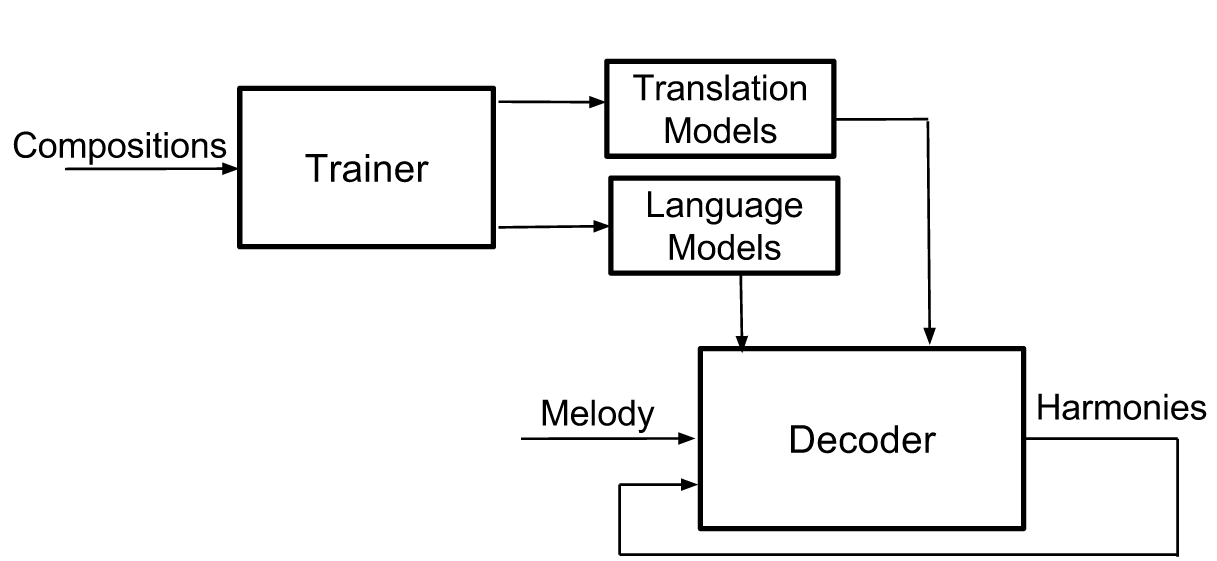
\includegraphics[scale=0.2]{design_overview.png}\\

Up until this point, we have only explained the model in terms of translating from the melody into one harmony voice. However, the goal is to produce $n - 1$ harmony parts for the given melody in order to produce a complete $n$-part arrangement. In order to do this, we view the translation portion of the system as a sequence of multi-source translations where the source languages are the melody voice and all of the harmony voices generated so far. The generated harmony voice will maximize the product of the probability given by its language model and the probabilities given by all the relevant translation models, where there is an individual translation model from each source voice to the voice being generated. More formally, given a set $S$ of source voices, the multi-source version of translation attempts to find a harmony line $H$ such that\\

$H = argmax_{H}p(H | M) = (\Pi_{S}\ p_{TM}(S | H)) \cdot p_{LM}(H)$.\\

Viewing translation as a sequence of steps then introduces the problem of determining the best order for the parts to be generated. Since each part is constrained by the parts generated previously, one would expect that the order in which the parts are generated will have an observable affect on the output. Indeed, our experiments have shown that the quality of the output varies greatly among different generation orderings. Details about how we plan to choose an optimal ordering will be discussed in the implementation section.

\section{System Implementation}
\label{sec:sys_implement}
\subsection{Programming Language}
Since we anticipated that the development of the system would involve a lot of experimentation, we decided to implement it in Python because of the language's ease of development and large amount of library resources, especially in the realm of machine translation and general NLP. Python's concise syntax, even when dealing with complex data structures, allowed us to focus on developing the core of our system.

\subsection{Data Collection and Interaction}
In order to train the language and translation models, we needed a large corpus of music data and a way to interact with it. For this,
we used third-party software called Music21 \cite{Cuthbert_music21:a}, a library developed at MIT which provides a simple interface for querying the library's database of musical scores. Music21 parses MusicXML, a type of encoding for standard music notation, into Stream objects, which can then be queried for any of the information contained in the notation including key, tempo, and notes with pitch and timing. Additionally, the Music21 package has over $2,000$ compositions, mostly written by classical composers. We have primarily trained on the package's Bach chorales, of which there are 402.

\subsection{Model Generation}
The translation and language models are implemented as nested dictionaries. The outer dictionary maps the given parameter, $A$, to the inner dictionary, which maps the unknown parameter, $B$, to the probability $P(B | A)$. In the case of the translation model, $A$ is a harmony note and $B$ is a melody note, while in the language model, $A$ is the sequence of $(i - 1) ... (i - n)$ harmony notes and $B$ is the $i^{th}$ harmony note.

The probabilities are calculated based on the counts of the events in the training compositions, plus smoothing techniques applied so that no event is assigned a zero probability. In this first iteration of explaining the probability calculation, we omit the smoothing techniques for the ease of explanation. Formally, the translation probabilities are given by:\\

$P(m_{i} | h_{i}) = \frac{count(m_{i} \wedge h_{i})}{count(h_{i})}$\\

and the language ngram probabilities are given by: \\

$P(h_{i} | h_{i - 1} ... h_{i - n}) = \frac{count(h_{i} \wedge h_{i - 1} \wedge ... \wedge h_{i - n})}{count(h_{i - 1} \wedge ... \wedge h_{i - n})}$\\

In the language model, to avoid any events having zero probability, we use LaPlace smoothing, also known as additive smoothing. Specifically, for some smoothing constant $\alpha$, the language ngram probabilities are given by: \\

$P(h_{i} | h_{i - 1} ... h_{i - n}) = \frac{count(h_{i} \wedge h_{i - 1} \wedge ... \wedge h_{i - n}) + \alpha}{count(h_{i - 1} \wedge ... \wedge h_{i - n}) + (48\alpha)}$\\

The constant $48$ in the equation above is meant to be the number of possible note values for the variable $h_{i}$. It is derived from the fact that there are 12 notes in each octave and that 4 is a very liberal estimate for how many octaves a particular voice can span. An alternate approach that we may experiment with would be to use, instead of $48$, the number of values for $h_{i}$ actually seen with the context $h_{i -1} ... h_{i - n}$, plus an additional $1$, for the ``unobserved'' note.

At the current point, the translation model is not smoothed because the system never considers generating harmony notes that were not seen with the input melody note in the training data. However, it is likely that that will change in the future, necessitating that we implement smoothing for the translation probabilties, probably similarly to how it has been implemented in the language model. 

Lastly, the values of the variables $n$ and $\alpha$ have so far been left unspecified because they are not yet finalized in the implementation. We intend to tune their values to maximize system performance on a cross-validation set of compositions. Their current values, however, are $n = 3$ and $\alpha = 1e-5$.

%TODO talk about how h ^ m events are determined (sounding at the same time)

\subsection{Note Representation}
We represent notes in the language and translation models as strings of pitch and octave number. Timing properties are currently not stored in the note representation because we have not yet integrated timing variation into the system. If timing were to be integrated, we propose adding an additional number to the end of the note's string representation describing the note's quarter length. For example, a whole note would have the number $4$ added to it's representation and an eighth note would have the number $0.5$ added to its representation. 

We also consider rests, moments of silence in the composition, to be ``notes'' in our model. They are represented by the string ``R''. Including rests makes it possible to harmonize a melody note with silence, thus offering some opportunity for rhythmic variation. However, including rests does pose a potential problem of producing too much silence, which is not optimal for music generation software. For example, imagine we are using a language model of n-gram size $2$, if $P(R | R)$ and $P (R | R R)$ are both relatively high, once we produce one rest, we may very well produce rests for the remainder of the song. Therefore, for fear of continually producing rests, we treat all contiguous sequences of rest symbols in a composition as one rest ``R'' in the model.

Measure bars are also modeled as ``notes'' our system. They are represented by the string ``BAR''. A special measure bar, the bar at the end of last measure in the song is given a special representation, ``END''. These notes are slightly different in that they are only present in our language model. ``BAR'' and ``END'' can only be harmonized with actual measure bars and song end in the given melody line, so there is no need to include them in the translation model. The motivation for including ``BAR'' and ``END'' in the language model is that they provide information about where in the composition the notes are being produced. Some notes may be more likely to start or end measures and some sequences of notes may be more likely to end a song. Coming back to the analogies between languages and musical voices, the ``BAR'' and ``END'' symbols can be likened to punctuation marks, which can give very strong cues about which words to generate, given that a string of natural language, a sentence for example, is about to end.

%TODO: talk about ngram size with bar and end included
\subsection {Decoder}
The goal of the decoder is to find the harmony line $H$ such that $H$ maximizes the probability of $P(H | M)$. However, the search space is much too large to enumerate all possible harmony lines in order to determine the best. Assuming the harmony voice spans no more than 4 octaves and that there are 12 notes in an octave, an exhaustive search of all harmony lines for a song with $n$ melody notes would require the inspection of $(12\cdot 4)^{n} = 48^{n}$ harmony lines. For an average length song comprised of $100$ melody notes, the number of possible harmony lines comes out to $48^{100} \approx 1.3e+168$. 

In light of this fact, we instead use a beam search decoder which only considers the top $k$ harmony line hypotheses generated. More specifically, at every iteration $t$, the decoder will have a set of hypothesis $S_{t}$ where each hypothesis is a sequence of $t$ notes, generated to harmonize with the input melody line, up to the $(t - 1)^{th}$ melody note. The decoder is begun with the set $S_{0}$ containing only the empty hypothesis. 

For each note in the melody, the decoder finds all possible harmony notes that can sound with that melody note, call it $m$. The harmony possibilities are just all the harmony notes $h$ s.t. $p(m | h)$ is in the translation model. Then the decoder constructs $S_{t + 1}$ by examining each hypothesis in $S_{t}$. For each hypothesis $hyp \in S_{t}$, a new hypothesis is constructed for each possible harmony note $h$, where the new hypothesis is just $h$ appended to $hyp$. All the new hypothesis generated in this iteration are added to $S_{t + 1}$. After all the new hypothesis have been added, the hypotheses in $S_{t + 1}$ are sorted in descending order by their $P(hyp | m_{0} ... m_{t})$ values, and only the top $k$ are saved for the next iteration.
The parameter $k$ will be tuned to maximize system performance while keeping time and space complexity in check. Currently, $k = 1000$.

%TODO:  Multi- Source (ways of combining translation models & deciding orders), Evaluation Metrics

\section{System Performance}
\label{sec:sys_perform}


\section{Remaining Work}
\label{sec:remaining_work}


\bibliographystyle{plain}     % Please do not change the bib-style
\bibliography{progress_report}  % Just the *.BIB filename

\appendix
\label{app}


\end{document} 

